\documentclass[aspectratio=169]{beamer}
\usetheme{default}

\usepackage[utf8]{inputenc}
\usepackage[ngerman]{babel}
\usepackage{graphicx}
\usepackage{csquotes}

\usepackage{lmodern}

%\usepackage{scrextend}
%\changefontsizes{18pt}

\usepackage[
backend=biber,
style=authoryear-ibid,
%sorting=ynt
]{biblatex}
\addbibresource{gravitropismus-bibliography.bib}

\author{Alexandra Smirnova}

\title{Präsentation zur Seminararbeit \hyphenquote{ngerman}{Gravitropismus}}
\subtitle{W-Seminar Biologie}

%\title{\hyphenquote{ngerman}{Gravitropismus}}
%\subtitle{Präsentation zum W-Seminar Biologie}

%\logo{}

%\institute{}

\date{19. Dezember 2018}

%\subject{}

\setbeamercovered{transparent}
%\setbeamertemplate{navigation symbols}{}
\setbeamertemplate{section in toc}[sections numbered]
\setbeamertemplate{subsection in toc}[subsections numbered]
\setbeamertemplate{caption}[numbered]


\useoutertheme{infolines}

\begin{document}
	\maketitle
	
	\begin{frame}
		\frametitle{Gliederung}
		\tableofcontents
	\end{frame}
	
	\section{Grundlagen von Gravitropismus}

	
	\begin{frame}
		\frametitle{Grundlagen von Gravitropismus}
		\begin{figure}[H]
			\centering 
			\includegraphics[width = 0.75\linewidth]{images/gravitrop_reagierende_Pflanze2.pdf}
			\caption{Gravitrop reagirende \emph{Arabidopsis thaliana} \parencite[5]{Masson2002}. Teilabbildung A zeigt den Zustand am Anfang, Teilabbildung B zeigt den Zustand nach vollzogener gravitropischer Reaktion. \label{gravitrop_reagierende_Pflanze}}
		\end{figure} 
	\end{frame}
	
	\subsection{Arten von Gravitropismus}
	
	\begin{frame}
		\frametitle{Arten von Gravitropismus}
		Positiv gravitrop - zur Schwerkraftquelle hin (nach unten zur Erdmitte)
		
		Negativ gravitrop - von der Schwerkraftquelle entgegengesetzt (nach oben)
		
		Transversalgravitrop - entweder horizontal oder quer nach unten in einem bestimmten Winkel 
		
	\end{frame}
	
	\subsection{Prozess der gravitropischen Krümmung}
	
	\begin{frame}
		\frametitle{Prozess der gravitropischen Krümmung}
	\end{frame}
		
	\subsubsection{Reizaufnahme bei Pflanzen}
		
	\begin{frame}
		\frametitle{Reizaufnahme bei Pflanzen}
		\begin{figure}[H]
			\centering 
			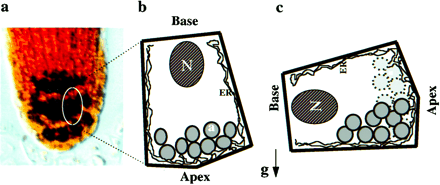
\includegraphics[width = 0.75\linewidth]{images/Statolithen2.png}
			\caption{Statolithen \parencite[345]{Chen1999}. Teilabbildung a zeigt eine Mikroskopaufnahme von Statolithen bei \emph{A. thaliana}. Teilabbildungen b und c zeigen die gravitrope Wirkungsweise von Statolithen, die auf Umlagerung der Amyloplasten bei Veränderung des Schwerkraftvektors beruht. \label{Statolithen}}
		\end{figure} 
	\end{frame}
			
	\subsubsection{Signaltransduktion}
		
	\begin{frame}
		\frametitle{Signaltransduktion}
		Funktion des Calciums 
		
		Funktion des elektrischen Feldes
	\end{frame}
			
	\subsubsection{Differenzielles Wachstum}
		
	\begin{frame}
		\frametitle{Differenzielles Wachstum}
		
		Funktion der Auxine und Gibberelline
		\begin{figure}[H]
			\centering 
			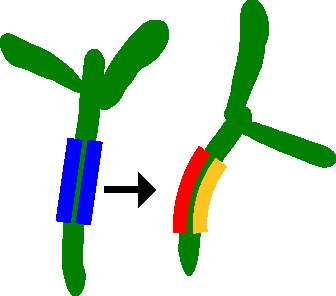
\includegraphics[width = 0.4\linewidth]{images/newdiff.pdf}
			\caption{Flanken wachsen ungleich nach der Signaltransduktion. Linkes Bild: Flanken gleich groß (blau); rechtes Bild: unterschiedliche Größe der Flanken (rot und orange).}
		\end{figure} 
	\end{frame}
	
	\section{Experimenteller Nachweis von Gravitropismus bei \protect\emph{Lepidium sativum}}
	
	\begin{frame}
		\frametitle{Experimenteller Nachweis von Gravitropismus bei \protect\emph{Lepidium sativum}}
	\end{frame}	
	
	\subsection{Methoden}
	
	\begin{frame}
		\frametitle{Methoden}
		\begin{figure}[H]
			\centering 
			\includegraphics[width = 0.5\linewidth]{images/IMG_1044.JPG}
			\caption{Vorbereitung des Experiments und vollständig aufgebautes Klinostat.\label{Klinostat2}}
		\end{figure}
		
	\end{frame}
	
	\subsubsection{Pflanzen, Material und Geräte}

	\begin{frame}
		\frametitle{Pflanzen, Material und Geräte}
		Pflanzen - \protect\emph{Lepidium sativum}
		
		Klinostat
		
		Weitere Materialien: Anzuchtbehälter, Säckchen aus Stoffstück, Plastiktüte, Messzylinder aus Plastik, diverse Gegenstände (z.B. Holzwürfel) 
	\end{frame}
	
	\subsubsection{Versuchsmethodik}
	
	\begin{frame}
		\frametitle{Versuchsmethodik}
		Pflanzengruppe 1: Kontrollgruppe
		
		Pflanzengruppe 2: Säckchen am Klinostat
		
		Pflanzengruppe 3: Anzuchttopf kopfüber
		
		Pflanzengruppe 4: Anzuchttopf horizontal am Boden
		
		Pflanzengruppe 5: Anzuchttopf mit Winkel zum Boden 
		
	\end{frame}
	
	\subsection{Durchführung und Ergebnisse}
	
	\begin{frame}
		\frametitle{Durchführung und Ergebnisse}
		
		Versuchstag 1 (28.05.2018): Vorbereitung
		
		Versuchstage 2–4 (29.–31.05.2018): Ankeimen
		
		Versuchstage 4–5 (31.–01.06.2018): Klinostat-Experiment mit Pflanzengruppe 2
		
		Versuchstage 6–7 (02.–03.06.2018): Ausrichtungs-Experiment mit Pflanzengruppe 3-5
	\end{frame}
	
	\subsubsection{Vorbereitung, Ankeimen}
	
	\begin{frame}
		\frametitle{Vorbereitung, Ankeimen}
	\end{frame}
	
	\subsubsection{Klinostat-Experiment}
	
	\begin{frame}
		\frametitle{Klinostat-Experiment}
		
			\begin{figure}[H]
			
			\centering
			\begin{subfigure}[b]{0.44\textwidth}
				\includegraphics[width=\textwidth]{images/IMG_1083.JPG}
				\caption{Sprossen vor Beginn des Klinostat-Experiments.\label{Foto 1}}	
			\end{subfigure}
			
			\begin{subfigure}[b]{0.44\textwidth}
				\includegraphics[width=\textwidth]{images/IMG_1073.JPG}
				\caption{Sprossen nach Abschalten des Klinostats.\label{Foto 2}}
			\end{subfigure}
			\caption{Klinostat-Experiment, Pflanzengruppe 2.\label{Foto 2}}
			
		\end{figure}
		
	
		
	\end{frame}
	
	\subsubsection{Ausrichtungs-Experiment}
	
	\begin{frame}
		\frametitle{Ausrichtungs-Experiment}
	
	\end{frame}
	
	\subsection{Diskussion und Fazit}
	
	\begin{frame}
		\frametitle{Diskussion und Fazit}
\end{frame}	
	

\end{document}